\chapter{Design}
\section{Overview}
\subsection{Key requirements}
The main focus of development was to design a professional looking, easy to use and eye-catching device for demonstration purposes such as info days. The following key requirements have been chosen:

\begin{itemize}
    \item Single power adapter or power cable (e.g. no need of labor power supplies) 
    \item Easy to install (e.g. montage on a camera tripod)
    \item Intuitive to operate via state-of-the-art graphical user interface
    \item Multiple audio streaming sources such as Bluetooth and USB input devices
    \item Great scalability and flexibility of the hardware and software design
\end{itemize}


\subsection{Key decisions}
was wird wo gemacht, FPGA, Raspi, etc...

\newpage
\section{Hardware Design}
The hardware of the Audio-Beamformer was designed using Altium Designer 22. The integrated 3D \acrshort{cad} functionality simplified the overall development and lowered the possibility of errors in the design.
The hardware has been improved over several iterations until a final version could be built. \newline
The 2-Layer \acrfull{pcb} with the size of 300.0\,mm\;x\;376.0\,mm has been manufactured and assembled by JLCPCB.\newline

\todo[inline]{Photo or render of PCB}


\newpage
\subsection{Block Diagram}
\begin{figure}[h!]
	\centering
	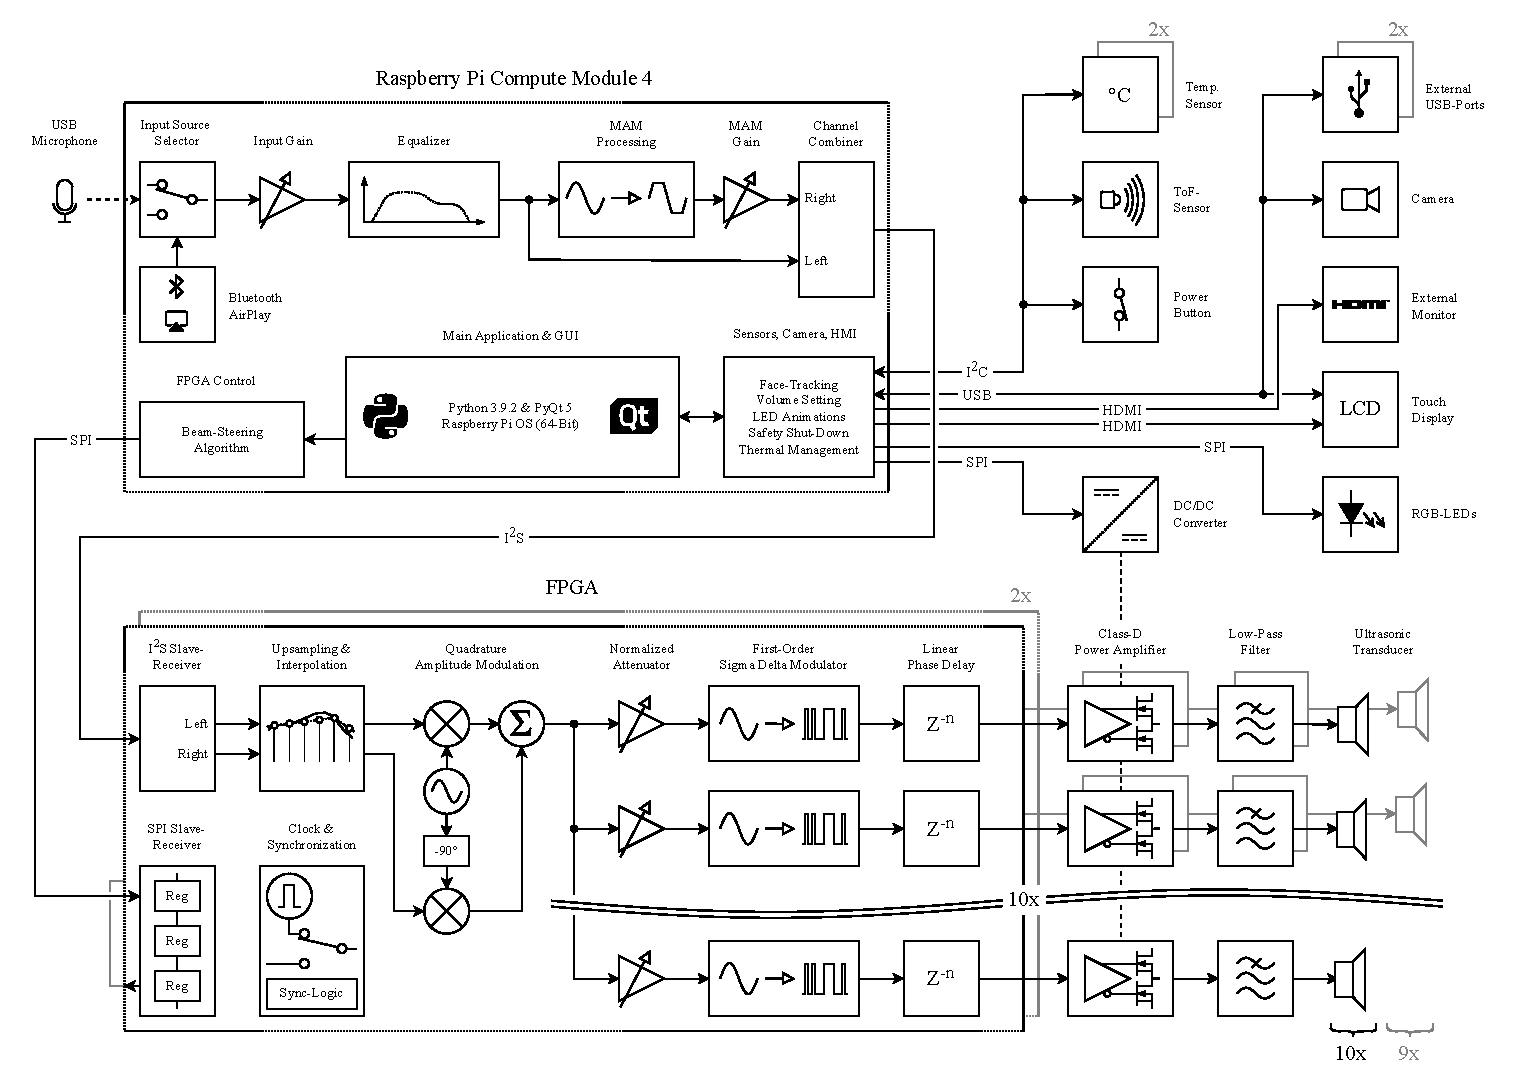
\includegraphics[width=21.5cm, angle=90]{images/4_Design/Hardware/System Block Diagram 2.pdf}
	\vspace{-0.2cm}
    \caption{Hardware Block Diagram}
    \label{fig:hardware-block-diagram}
\end{figure}

\clearpage
\subsection{Power Management}
The Audio-Beamformer is powered directly by mains voltage. As a connector, the widely used C14 (IEC 60320) has been chosen. Because of the metallic casing, protective earth is required. It has been connected directly to the back panel. The main switched mode power supply is made by \textit{Mean Well} and delivers 48\,V \acrshort{dc} and up to 163\,W output power. The LSP-Series is specially designed for low-profile applications and therefore ideal in this use case.\newline
The simplified power management diagram \ref{fig:simplified-power} provides a better overview of how each voltage rail is created.

\begin{figure}[h!]
	\centering
	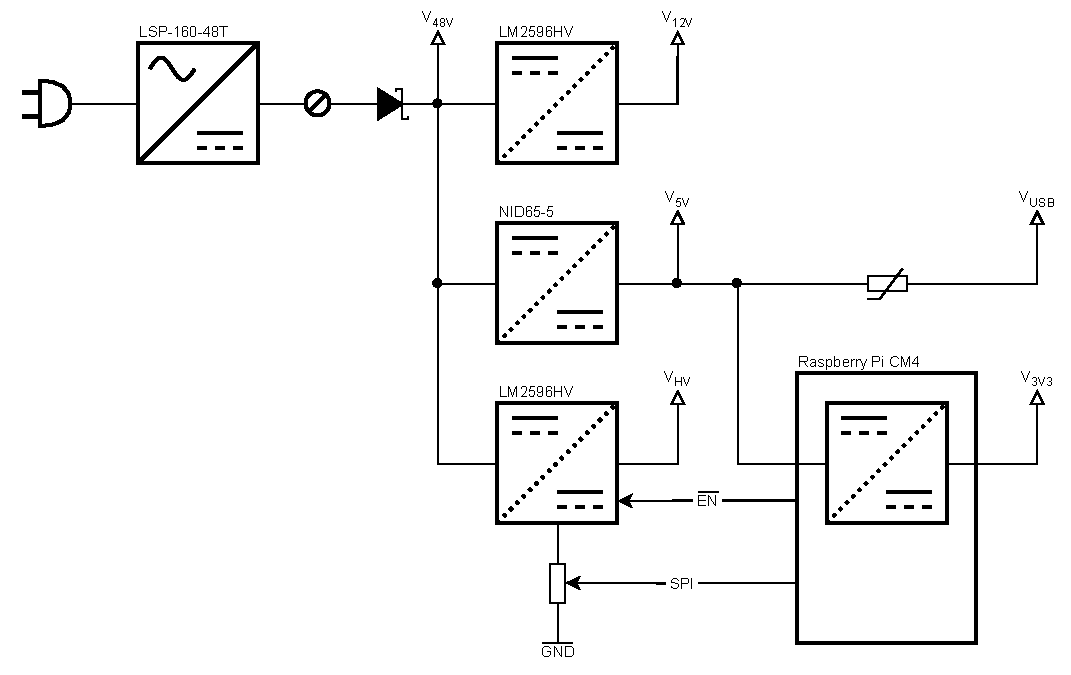
\includegraphics[width=\textwidth]{images/4_Design/Hardware/Power Supply Overview.pdf}
	\vspace{-0.6cm}
    \caption{Simplified Power Management}
    \label{fig:simplified-power}
\end{figure}

As a reversed polarity protection a schottky diode has been placed directly after the input connector. Further \acrshort{dc}-\acrshort{dc} buck converters generate fixed 5\,V (6.5\,A), 12\,V (2.0\,A) and a variable HV rail.


\bigskip
\begin{wrapfigure}{r}{7cm}
    \vspace{-0.6cm}
    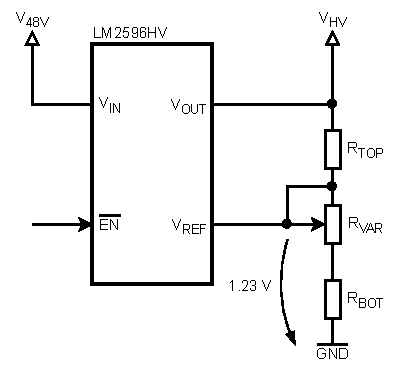
\includegraphics[width=7cm]{images/4_Design/Hardware/Variable Buck-Converter.pdf}
    \vspace{-0.6cm}
    \caption{Variable Buck-Converter}
    \label{fig:variable-buck-converter}
\end{wrapfigure} 
For adjusting the physical output volume of the ultrasonic transducers, the amplifier drive voltage must be changed accordingly. The HV voltage supply can be set between 5.2\,V and 23.5\,V (2.0\,A). This has been achieved by using a digital potentiometer (MCP41010T) which is controlled by an \acrshort{spi}-Interface.\\
For safety reasons, the HV voltage is turned off per default and must be enabled by a physical logic signal provided by the Raspberry Pi.
\clearpage

The output voltage can be calculated as follows:

\begin{equation}
    V_{HV}(R_{var}) = \frac{V_{ref}}{R_{bot} + R_{var}} (R_{bot} + R_{top} + R_{var})
\end{equation}

Where $R_{var}$ is proportional to its 8-bit value (\codeword{0x00} $\cong$ 0\,$\Omega$ and \codeword{0xFF} $\cong$ 10\,k$\Omega$). The reference voltage of the DC-DC buck converter (LM2596HV) is 1.23\,V. The resistor values used in the design are $R_{top}$ = 39\,k$\Omega$, $R_{bot}$ = 2.0\,k$\Omega$ and $R_{var}$ = 10\,k$\Omega$. This leads to the following approximation:
 \begin{equation}
    V_{HV}(d) \approx 5.2\,V + d\:\frac{20\,V}{255}
\end{equation}

\subsection{Raspberry Pi Compute Module 4}
As a main processing platform the Raspberry Pi Compute Module 4 has been chosen due to its powerful quad-core processor and the great software support based on a large community. The exact model used in the design has 4\,GB of \acrshort{ram} and fixed installed 16\,GB of embedded \acrshort{emmc} flash storage. This has the advantage of being more reliable than systems that are dependent on a \acrshort{sd}-Card.
To increase the performance, the Raspberry Pi has been overclocked to 1.0\,GHz. Sufficient cooling is provided by a heat sink and four cooling fans.
The \acrshort{io} operating voltage has been set to 3.3\,V.

\subsection{FPGA} \label{hardware_fpga}
There are two \acrshort{fpga}s used in the design for generating the drive signals for the ultrasonic transducers. Each \acrshort{fpga} is mounted on a development board called \textit{Alchitry Cu}. They are installed as daughter-boards on the main \acrshort{pcb} by high-speed board-to-board connectors. Both \acrshort{fpga}s receive the audio stream via an \acrshort{i2s}-Stream and get controlled by a simple \acrshort{spi}-Protocol in an daisy-chain configuration. More details on this in section \ref{fpga_i2s} and \ref{fpga_spi}.\\
The \acrshort{fpga} boards are powered by 5\,V, because they have an on-board 3.3\,V regulator build-in.


\subsection{Sensors and HMI}
The Audio-Beamformer contains several sensors that are connected by different interfaces to the Raspberry Pi Compute Module. The \acrfull{hmi} enables easy access to change various settings of the device.

\subsubsection{Camera}
To be able to direct the sound towards a specific person, a camera is needed. In this case a \acrshort{usb}-Camera has been chosen since it is easy to connect and does not need any special device drivers. The type \textit{ELP-USB500W02} provides a resolution of 1280\,x\,720 pixels and a frame rate of up to 30\,FPS. The optics used in this application are designed to match the viewing angle of the camera to the maximal beam-steering angle of the Audio-Beamformer. In this particular case, a camera lens with a focal length of \todo{check}\,mm has been chosen which results in a viewing angle of ca. ±40°.

However the camera had to be slightly modified. On startup, it tries immediately to establish an \acrshort{usb} connection to the host device. If there is no response during the first 500\,ms the camera goes into a power-down/suspend mode. In this state it can't be recognized by the host until it gets power-cycled. This issue has been solved by increasing the RC time constant of the camera internal power-on reset circuitry from 4.7\,ms to ca. 4.7\,s. In addition a schottky diode has been added to guarantee a fast discharge time after powering off the device. This ensures a valid reset-pulse even if the device gets power-cycled very rapidly.

\begin{figure}[h!]
    \centering
    \subfloat[\centering Reset-Circuit]{{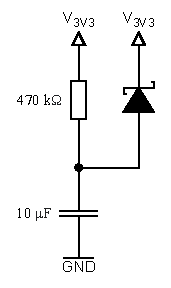
\includegraphics[height=6cm]{images/4_Design/Hardware/Camera Reset-Circuit.pdf}}}
    \qquad
    \subfloat[\centering Location of RC-Circuit]{{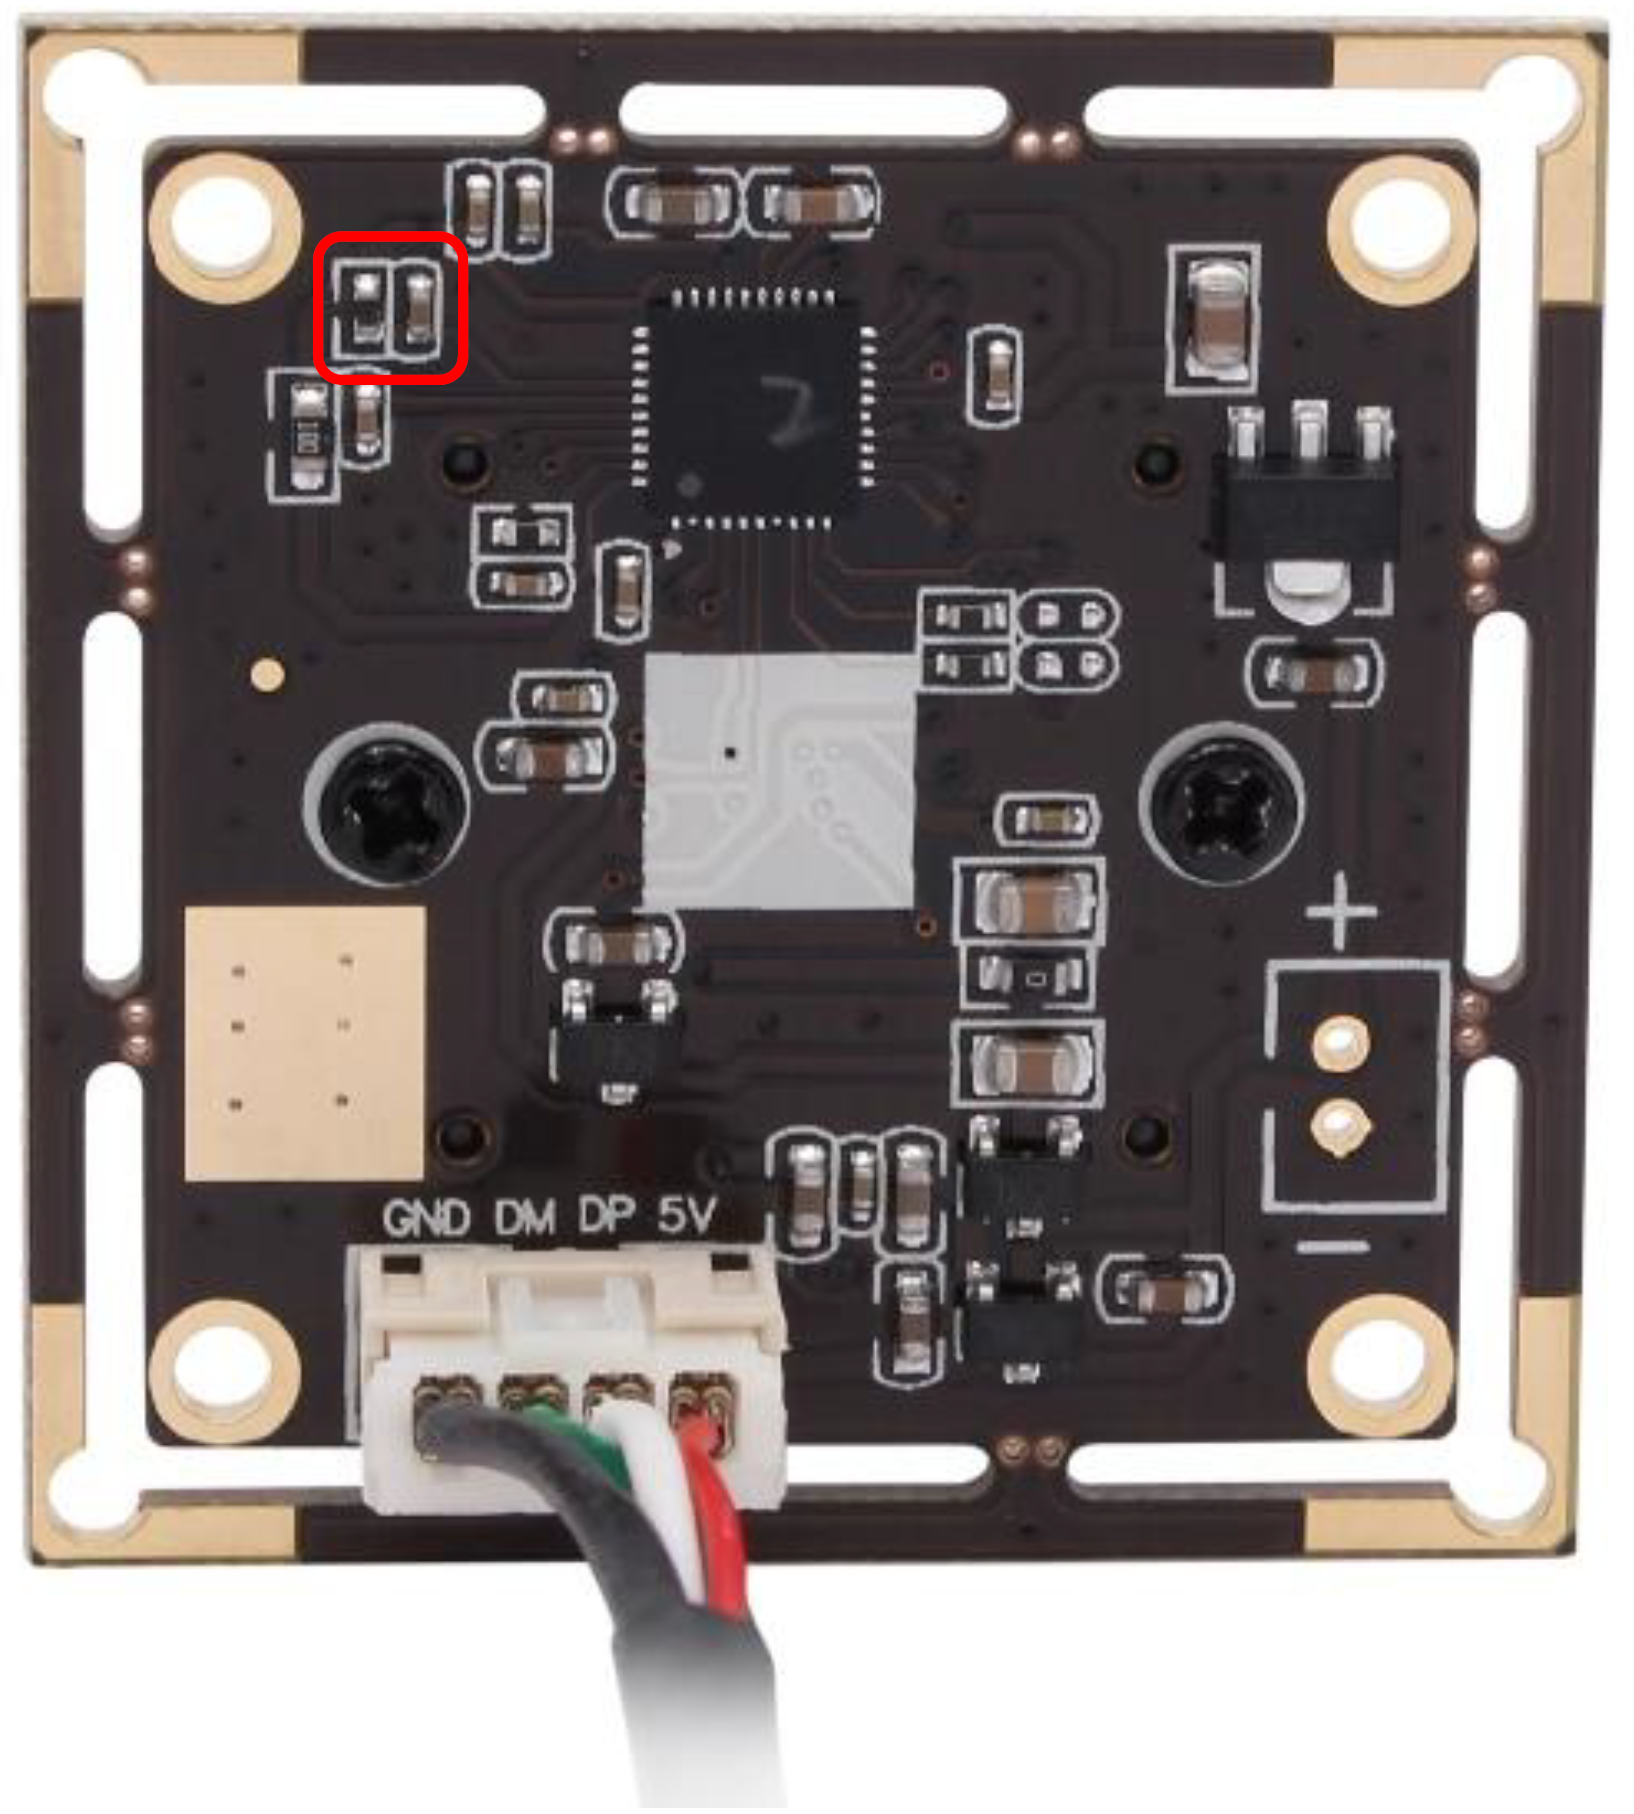
\includegraphics[height=5.5cm]{images/4_Design/Hardware/Camera-Modification.PNG}}}
    \caption{Camera Modification}
    \label{fig:camera-modification}
\end{figure}


\subsubsection{Temperature Sensor}
There are two temperature sensors embedded on the \acrshort{pcb}. One to measure the ambient temperature (and therefore be able to calculate the speed of sound in air according to the temperature, described in \ref{4_Sensors_Speed-of-sound}) and the second-one to measure the system temperature which is used to control the speed of the four \acrshort{dc}-Fans. The temperature sensors used in the design are of the type \textit{TMP112} made by Texas Instruments. They have an accuracy of ±0.5\,°C and are connected to the \acrshort{i2c}-Bus of the system with individual IDs (\codeword{0x48} \& \codeword{0x49}). The temperature gets read every 500\,ms.

\subsubsection{Time-of-Flight Sensor}
For various safety reasons it is important to turn off the speaker output when a person enters the near-field of the Audio-Beamformer (d $<$ 1\,m). This safety mechanism has been realized by using a multi-zone \acrfull{tof} sensor. The \textit{VL53L5CX}, made by ST Microelectronics is specially designed for a wide field of view (63°). It can measure distances up to 4\,m and has a resolution of 8\,x\,8 zones. It is connected to the \acrshort{i2c}-Bus and can be address by the ID of \codeword{0x52}. The internal update rate has been set to 5\,Hz to minimize traffic on the \acrshort{i2c}-Bus. To further increase the data throughput, the \acrshort{i2c} clock rate has been set to 1\,MHz.

The distance-map data then gets further processed as described in section \ref{4_Sensors_Near-field}.

\newpage
\subsubsection{Rotary Encoder}
To easily adjust the volume of the Audio-Beamformer, a pushable rotary encoder has been placed below the display. Pressing the knob toggles the mute state of the output stage. This becomes very handy if the volume level should stay the same, but the speaker needs to be turned off temporarily. Both, the volume level and the mute state can be overwritten in the \acrshort{gui}. This is can only be achieved by the relative position measurement of rotary encoders and would not be possible with ordinary potentiometers.

To suppress contact bouncing and thus prevent false inputs, a simple RC debouncing circuit with a schmitt-trigger buffer has been installed.

\subsubsection{Power-Button and Cooling-Fans}
On the right side of the Audio-Beamformer, a 22\,mm stainless steel push button has been installed to power-on and off the Raspberry Pi Compute Module 4. The integrated \acrshort{rgb}-\acrshort{led} ring is driven by a specialized \acrshort{pwm}-Driver \acrshort{ic} with \acrshort{i2c}-Interface. The \textit{PCA9633DP1}, made by Texas Instruments provides four individual addressable 8-Bit \acrshort{pwm} channels and is addresses at the \acrshort{i2c}-Address of \codeword{0x62}. \acrshort{pwm}-Channel 1, 2 and 3 are used for the red, green and blue \acrshort{led}s of the bush button, while channel 0 is connected to the four \acrshort{dc}-Fans installed in the back of the enclosure. The Fans are wired in parallel and operate at a maximal voltage of 12\,V.\\
The system temperature is used to control the speed of the cooling fans. They start running at a temperature of 40\,°C and provide proportional air flow as the temperature increases. At 60\,°C the operate at full speed.

\subsubsection{LCD Touchscreen}
Since the beginning of the project, the idea was to create an attractive and modern looking device. One of the key components is the large \acrshort{lcd} touchscreen. It has a diagonal size of 11.9\,inch and a resolution of 1480\,x\,320 pixels. As interface, \acrshort{hdmi} is used for the video stream and \acrshort{usb} to transmit the touch-screen data to the Raspberry Pi Compute Module 4. Important to notice is, that the corners of the display are rounded (radius of 5\,mm), this has been considered when designing the \acrlong{ui}.

\subsubsection{RGB-LEDs}
To present a visual feedback of the current beam-steering angle and the active window-function, each row of the array contains one individually addressable \acrshort{rgb}-\acrshort{led} on top and on the bottom of the ultrasonic transducers. The type of those intelligent \acrshort{led}s is called \textit{APA102}. They embed an integrated driver \acrshort{ic} which can be controlled via a non-standard \acrshort{spi} protocol (special start and end sequence instead of a chip select line) in a daisy-chain configuration. The LEDs have a physical size of 5.0\,x\,5.0\,mm and are directly powered by the 5\,V voltage rail.\\
Next to the 38 \acrshort{led}s used for the array channel illumination, further 20 \acrshort{led}s are placed on a ring around the camera. This offers direct visual insight of the face-tracking algorithm. While a person is tracked, the \acrshort{led}s are animated in a "breathing" brightness motion. When there is no face detected, a spinning gradient animation is shown.\\
The maximal power consumption is about 25\,W if all \acrshort{led}s are fully turned on.

\subsubsection{External Interfaces}
The Audio-Beamformer can easily be connected to an external display by using the \acrshort{hdmi}-Port on the left side of the enclosure. In combination with the two spare \acrshort{usb}-Ports, e.g. for connecting a keyboard and mouse, the system can easily be debugged. Even developing new software features directly on the target platform is possible. To back-up the data of the \acrshort{emmc} flash storage on the Raspberry Pi Compute Module 4, a  \acrshort{usb} Type-C Port has been added. To start the back-up procedure, the tiny slide switch next to the \acrshort{usb}-C Port must be set to the up-position. This enables the bootloader of the Raspberry Pi Compute Module 4 on power-up of the device. When connected to an external host (such as a computer), the Audio-Beamformer gets recognized as a mass-storage-device. A back-up tool like e.g. \textit{Win32DiskImager} can be used to create a binary image of the operating system inclusive all user data.

\subsection{Output Stage}
The output stage represents a Class-D design in a MOSFET full-bridge configuration. This topology has the advantage of high efficiency and low part count. However, the proper design of such output amplifiers has its difficulties. Specially when operated at high switching frequencies (3.125\,MHz in this case), transient turn-on and turn-off times must be very short. This can lead to ringing and voltage spikes on the output signal.
MOSFETs are known to be very sensitive when it comes to such transient voltage spikes. Exceeding the maximal Drain-Source voltage will likely result in a breakdown and a permanent short circuit. To prevent such behavior, several options can be considered:

\begin{itemize}
    \item Utilize MOSFETs with higher voltage rating
    \item Reduce switching speed and therefore increase transient time
    \item Impedance matching of load and driving source (e.g. with series resistor)
    \item Introducing passive dampening networks, such as RC-Snubber circuits
\end{itemize}

MOSFETs with higher Drain-Source voltage ratings have typically more gate capacitance and therefore would lead to a drastically higher switching current. A great compromise has been found with the type \textit{BSS123}, it has a Drain-Source voltage rating of 100\,V and can withstand a continuous current of 200\,mA. The gate capacity is around 32\,pF (at a gate voltage of 12\,V). 

As mentioned above, RC-Snubber networks can help to suppress voltage spikes by creating a low-impedance path for the current, circling in the low-side of the half-bridge. Figure \ref{fig:rc-snubber} shows how important a sufficient bypass capacitor is to stabilize the high-side. Texas Instruments published a very comprehensive guide on how to design such RC-Snubber networks \cite{ti_class_d_snubber_design}.  

\begin{figure}[h!]
	\centering
	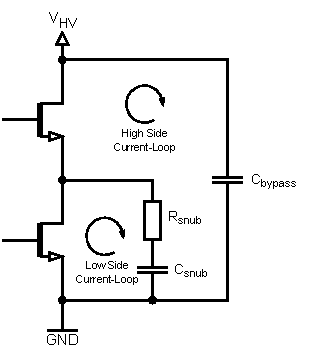
\includegraphics[width=6cm]{images/4_Design/Hardware/Class D Snubber.pdf}
	\vspace{-0.2cm}
    \caption{Class-D Half-Bridge with RC-Snubber}
    \label{fig:rc-snubber}
\end{figure}

\todo[inline]{write about output filter inductor selection}

\pagebreak
\subsection{Ultrasonic-Transducer Array}
Achieving a decent array size is important to get a better directivity, higher output volume and in general greater beam-steering properties. Thus a large amount of ultrasonic transducers is needed. In order to keep the cost down of the project, one of the key criteria was the unit price. Directly ordering by professional suppliers, such as Digikey, Mouser, Farnell, etc. results in very high prices of more than 7\,CHF per piece. This was not acceptable since more than 150 pieces are needed in the final design. Fortunately it was possible to get directly in touch with a manufacturer based in China. The datasheet of the \textit{MA40A16} (attached in the appendix \ref{appendix_ma401a6}) has been studied firmly, with the conclusion that the type is suitable for this project and satisfies all key parameters. The price per unit is only 0.3\,CHF.\\
They operate at a resonant frequency of 40\,kHz and have physical diameter of 16\,mm. Important to notice is, that the metal case makes electrical contact to one of the pins. Thus it's important to leave enough clearance between the transducers to prevent short circuits.

\subsubsection{Arrangement \& Placement}
As prior analysis showed, the denser an array can be built, the better is it's performance. Due to the circular shape of the ultrasonic transducers, the optimal arrangement is a hexagonal pattern. This has some further advantage of creating a smaller horizontal spacing between each row of ca. 14.75\,mm (when a diagonal distance of 17.0\,mm is chosen with a gab of 1\, mm between the transducers). In general, a smaller spacing leads to higher efficiency and a better beam pattern (e.g. less dominant side lobes).\\
The final number of 19 rows has been the result of several considerations. First of all, the row count must be odd, to create a symmetrical design with only one centre row. Further the total width of the array must comply with the maximal manufacturing and assembly size of \acrshort{pcb}s by JLCPCB (max. 480\,x\,320\,mm). And at last, the overall dimension should match the size of the display to create a cleaner visual impression of the final design. At some point, adding more rows to the array will not lead to any further audible improvements. This is mainly caused by the window-function which tends to strongly reduce the gains of the rows at both ends of the array.\\
A row height of 8 has been chosen to create stronger beam-characteristics, specially in the vertical direction. In addition, the parallel wiring of multiple ultrasonic transducers lowers the total impedance, which has the advantage of operating at a lower driving voltage to create the same amount of power.

\newpage
\section{FPGA Design}
As mentioned in Section \ref{hardware_fpga}, the \textit{Alchitry Cu} \acrshort{fpga}-Board has been used. The specific chip is called \textit{iCE40-HX8K}, made by Lattice Semiconductor. It offers a total of 7680 logic cells, 32 blocks of dual-port \acrshort{ram} (4\,KBit each), two independent \acrshort{pll}s and 79 \acrshort{io}-Pins. It is operated at 100\,MHz which is more than enough for this application.

To keep the design process as efficient as possible, a development environment has been chosen which is easy to use and offers lots of predesigned \acrshort{ip}-Blocks. Namely the \textit{IceStudio} has been used in combination with the open source tool-chain called \textit{IceStorm} which currently supports all \acrshort{fpga}s of the iCE40-Family.\\
The tool offers a combination of a graphical design work-flow with the option of embedding custom blocks of Verilog code. Due to the open source nature, lots of individuals published extension libraries of hundreds of \acrshort{ip}-Blocks. This became very handy, specially for integer arithmetic operations, such as addition and multiplication.



\newpage
\subsection{Block Diagram}
\begin{figure}[h!]
	\centering
	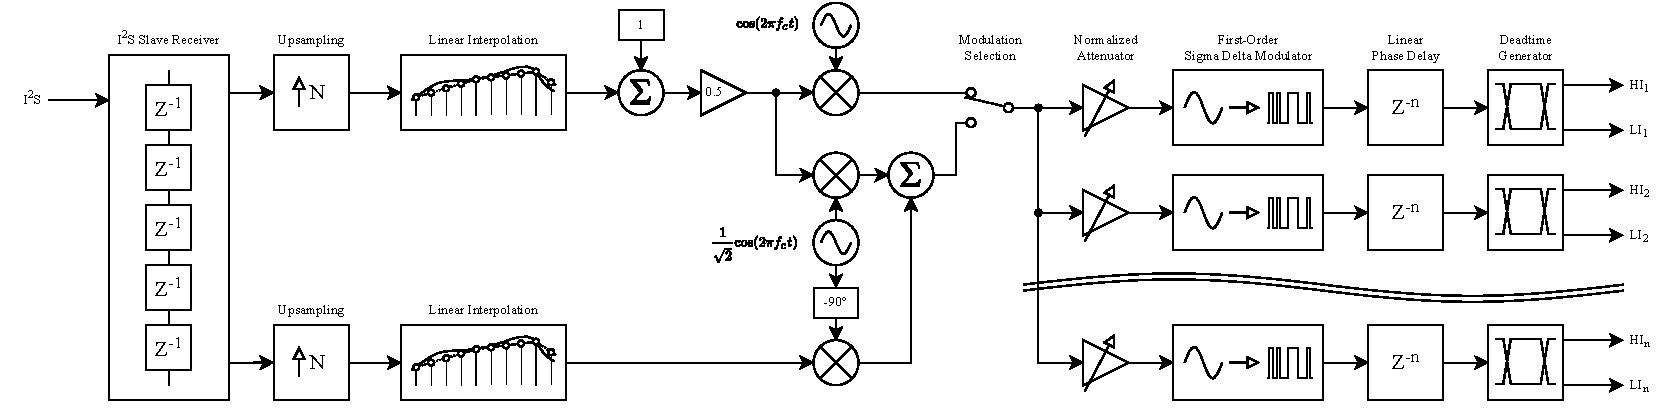
\includegraphics[width=22.2cm, angle=90]{images/4_Design/FPGA/FPGA Block Diagram.pdf}
	\vspace{-0.2cm}
    \caption{FPGA Signal Flow Diagram}
    \label{fig:fpga-signal-flow}
\end{figure}

\subsection{Clock \& Synchronization}
Making sure that both \acrshort{fpga}s run simultaneously and don't drift apart in time, the system clocks must be shared. This means that one of the \acrshort{fpga}s acts as a master, which provides a clock signal to all slaves. In order to use the same logic configuration, a dedicated ID-Pin has been added to differentiate the master (logic level 0) and slave (logic level 1) configuration.\\
In addition, a synchronization pulse gets created by the Raspberry Pi Compute Module 4 at the startup of the device. This signal is used to reset the local oscillators on all \acrshort{fpga}s, to make sure that the phase of the carrier signal is in sync.



\subsection{I\textsuperscript{2}S} \label{fpga_i2s}
\subsection{SPI} \label{fpga_spi}
\subsection{Interpolation}
\subsection{Modulation}
\subsection{Sigma-Delta-Modulator}
\subsection{Channel Delay \& Gain}
\subsection{Dead Time Generator}


\section{Software Design}
The software on the Raspberry Pi was written in Python, due to its simplicity. 
\subsection{Structure}
\subsection{GUI}
The GUI was made with PyQt, which is a wrapper for Qt in python. The main goals where to create an intuitive, easy to use and informative graphical user interface. 
The three main sections of the UI can be reached through the buttons on the left. We decided to separate the configurable parameters into three sections, processing, channels and settings. General settings such as mute, volume and output level are always present on the right side of the screen. 
\subsubsection{Processing}
The processing window is divided into five different sections. All of these sections contain settings for the audio processing.
\begin{enumerate}
    \item Source \\
    In this section the audio input source and input gain can be adjusted. To get a direct visual feedback of the input sound level a gauge was added.
    \item Equalizer \\
     In the second section the equalizer can be enabled and can be chosen from preset list. To give more information about the current equalizer used a bode plot can be seen at the bottom. 
    \item Interpolation \\
    In this section the interpolation can be enabled and the oversampling rate can be chosen. The oversampling values are 2, 4, 8, 16, 32, 64.
    \item Modulation type \\
    In the last section the modulation type can be chosen. Additionally if the modulation type chosen is MAM a gain for the distortion channel can be set. 
\end{enumerate}

\begin{figure}[h!]
    \centering
    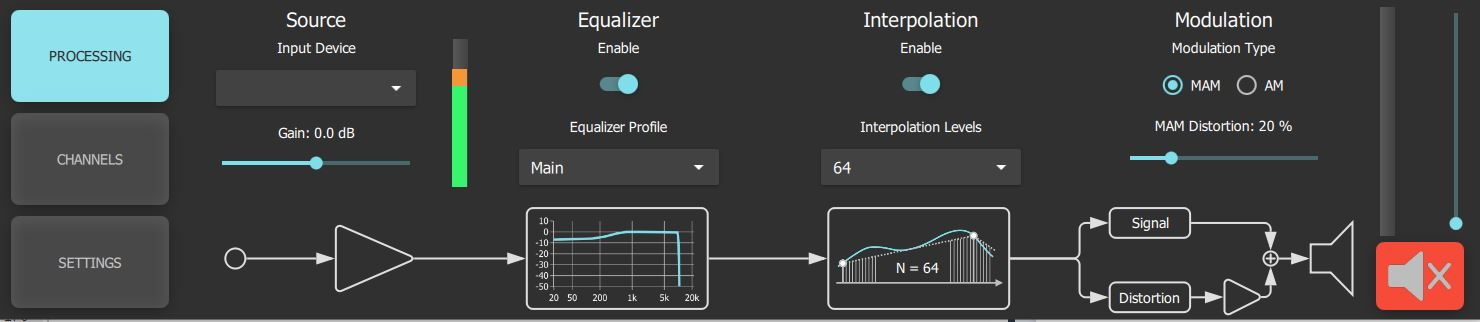
\includegraphics[width=\textwidth]{images/4_Design/GUI_Processing.JPG}
    \caption{GUI Processing View}
    \label{4_fig:gui_processing}
\end{figure}

\subsubsection{Channels}
The channels window is split up into 3 different areas.
\begin{enumerate}
    \item Beamsteering \\
    In this section the beamsteering can be enabled and the angle source can be set. If the angle source is set to "Camera" the face tracking is activated, else if it is set to "Manual" a slider appears with which the angle can be set manually. The last angle source is "Pattern" for which a predefined pattern which the angle should be is used. 
    \item Window \\
    In this section the window function can be enabled. If it is disabled the window "Rectangle" is used. To give more information about the current window function selected a plot of how the gains are set is shown at the bottom. 
    \item Video feed \\
    In this video feed one can see who is currently being detected and tracked. If a light blue window surrounds a face this is the current tracked face. If it is grayed out a face was detected but is currently not tracked.
\end{enumerate}
\begin{figure}[h!]
    \centering
    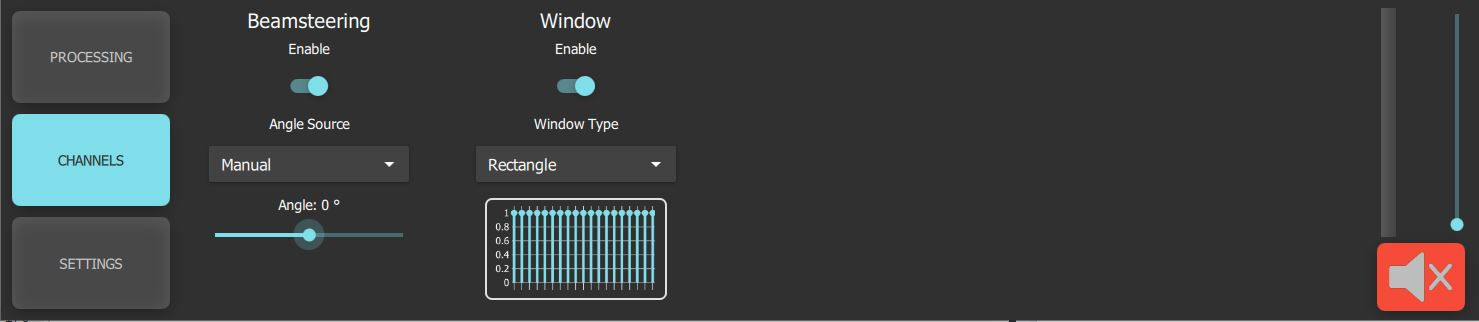
\includegraphics[width=\textwidth]{images/4_Design/GUI_Channels.JPG}
    \caption{GUI Channels View}
    \label{4_fig:gui_channels}
\end{figure}

\subsubsection{Settings}
The setting page is split up into 6 different areas.
\begin{enumerate}
    \item LED \\
    In this section the LEDS can be enabled and their brightness can be set. 
    \item ToF Sensor \\
    In this section the ToF Sensor can be disabled and its sensitivity can be changed. To get a visual feedback of the sensitivity a gauge is present.
    \item Max volume \\
    With this slider the maximum volume which can be reached by the loudspeaker can be adjusted. This can be done if the device needs to be used inside to guarantee safety.  
    \item Beamfocusing \\ 
    In this section the beamfocusing can be enabled and the distance where the beams should meet can be adjusted. 
    \item Stats
    This section shows temperature and load information about the system and the CPU.
\end{enumerate}
\begin{figure}[h!]
    \centering
    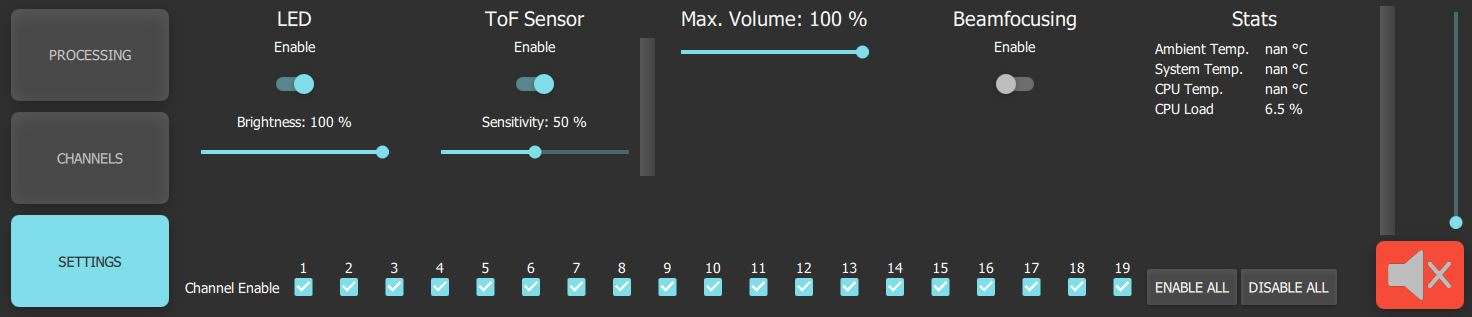
\includegraphics[width=\textwidth]{images/4_Design/GUI_Settings.JPG}
    \caption{GUI Settings View}
    \label{4_fig:gui_settings}
\end{figure}

\subsection{Audio Processing}
In this module the audio processing is made. First the audio input is read block based into the program then the audio is filtered through an equalizer and changed for the modulation and in the end it is outputted through $I^2S$ to the FPGAs.
\subsubsection{Audio stream}
The audio stream is implemented in python using a library called "Sounddevice", which wires the input to the output in a non blocking way. The audio is read block based with a block size of 8192. We tried to keep the block size as small as possible to guarantee low latency if a microphone is used. 
\subsubsection{Equalizer}
To compensate the distortion generated by the frequency response of the transducer, which is shown in Section \ref{6_sec:Frequency_response}, a FIR equalizer can be enabled between the input and the output of the audio stream. The equalizer that can be selected can be added into the file \todo{File verweisen} in the form \todo{Form for equalizer}. On start up a bode plot is created for each equalizer and stored in \todo{File path} for the GUI.
\subsubsection{Modulation type}
Currently the two modulation types implemented are AM and MAM. The difference between these two is that the second channel is in the case of MAM not an exact copy of the first channel but a second order approximation of the distortion term shown in Equation \ref{3_eq:mam_distortion_approx} 
\begin{equation}
    \text{Left Channel} = 1 - \frac{1}{2}i(t)^2 - \frac{1}{8}i(t)^4.
\end{equation}
Where $i(t)$ is the incoming audio signal. 
\subsection{Beam-Steering}
In the beam-steering modules delay and gain for all the channels are calculated and are adjusted using the SPI-Interface. 
\subsubsection{Delays}
The formula used for calculating the individual delays are
\begin{equation}
    \tau_m = m\frac{d}{c_0}\sin{\varphi},
\end{equation}
where d is the distance between the transducers, $\varphi$ the angle to steer to and $c_0$ the sound of speed. The sound of speed is also directly calculated in this module by using the ambient temperature input from the sensors module using the formula
\begin{equation}
    c_o = 331.5 + 0.607 \cdot T_{\text{Ambient}}
\end{equation}
The minimum angle which a phased array can reach is determined by the physical properties of the construction and by the smallest delay that can be applied to a signal. The physical properties of the transducer arrays are a spacing of $d=14.75mm$ and the numbers of channels $M=19$. The smallest delay in our case is $\tau_{min} = \frac{1}{6.25MHz} = 160ns$ and is determined by the output sampling rate
\begin{equation}
    \varphi_{min} = \arcsin{\left ( \frac{\tau_{min} c_0}{M d} \right ) } \approx  0.21^{\circ}.
\end{equation}
The maximal angle that can be reached is determined by the largest delay that can be applied to a signal. This is determined by the maximum number of memory cells, which in this case is $N_{MC} = 4092$, available for a channel on the FPGA. The largest delay that can be applied is $\tau_{max} = \tau_{min} \cdot N_{MC} \approx 654 \mu s $. Which leads to a maximal angle of 
\begin{equation}
    \varphi_{max} = \arcsin{\left ( \frac{\tau_{max} c_0}{M d} \right ) } \approx  53.4^{\circ}.
\end{equation}
\subsubsection{Gains}
For controlling the main lobe with and side lobe level different windows can be applied to the loudspeaker. In addition to the gain of the channel this also effects the brightness of the LEDs to give the user more information about the window. 
\subsection{Sensors}

\subsubsection{Near-Field Avoidance System} \label{4_Sensors_Near-field}
\todo[inline]{Include formula of processing distance map, wie detailliert wemmer das beschribe?}

\subsection{Face Tracking}
\subsubsection{MNN}
\subsection{Operating System}
\subsubsection{Linux}
\subsubsection{Bluetooth \& Airplay}


\section{Mechanical Design}
\subsection{Concept}
\subsection{Casing}
\newpage
